\chapter{数值计算方法}
为了实现对细长航行体进入波浪场的模拟,本文借助流体力学计算软件 Fluent 对不同的入水条件进行数值模拟。本文首先确定了计算的几何模型和区域,进行恰当的网格划分,给予合适的 UDF 边界条件,选用适当的数值方法,从而实现了波浪场的模拟。之后借助界面捕捉的 VOF 方法以及重叠网格技术,实现了航行体入水的方案设计。
\section{几何模型和网格划分}
本文为了模拟五级海况\cite{Xia1987}的环境,选取的环境场背景网格为 $300 \mathrm m \times 60 \mathrm m \times 10 \mathrm m$ 的长方体区域。模拟水深 $40 \mathrm m$,波长 $40 \mathrm m$,波高近 $3 \mathrm m$。由于水面附近的计算精度要求高,故以水面所在平面为最精细的网格,两侧以一定比例按等比数列扩大其网格间距。入水过程发生在波浪船舶方向的 $0 < x < 200$ 范围内,后半区域 $200 < x < 300$ 为消波区。工作区划分为均匀网格,每个波长内大约80个网格,消波区采用快速增大的粗糙网格,总体网格量为84万,可以足够精细地描述波浪场环境。

运动网格为围绕入水细长航行体的圆柱体网格。细长航行体的长度$5 \mathrm m$,直径$0.5 \mathrm m$。网格沿圆柱体轴线方向采用等距划分,沿径向方向从外至内按照等比数列距离缩小,以增强靠近物体表面部分的精度。在模拟过程中,动网格始终环绕着入水物体,与入水物体之间的相对位置保持不变,并使用重叠网格技术以进行区域内的数值模拟。在初始状态下,背景网格与运动网格如图~\ref{fig:overlay_grid}所示

\begin{figure}[!htp]
  \begin{subfigure}{\textwidth}
    \centering
    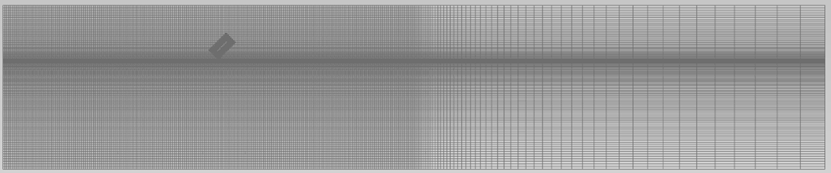
\includegraphics[]{overlay_grid.png}
    \caption[]{入水角度 $45 ^ \circ$ 的初始重叠网格}
  \end{subfigure}

  \quad

  \begin{subfigure}{0.3\textwidth}
    \centering
    \includegraphics[width = \textwidth]{fig/mesh/WaterEntry-AOA45.jpg}
    \caption[]{$45 ^\circ$ 的局部网格}
  \end{subfigure}
  \hspace{0.2cm}
  \begin{subfigure}{0.3\textwidth}
    \centering
    \includegraphics[width = \textwidth]{fig/mesh/WaterEntry-AOA60.jpg}
    \caption[]{$60 ^\circ$ 的局部网格}
  \end{subfigure}
  \hspace{0.2cm}
  \begin{subfigure}{0.3\textwidth}
    \centering
    \includegraphics[width = \textwidth]{fig/mesh/WaterEntry-AOA90.jpg}
    \caption[]{$90 ^\circ$ 的局部网格}
  \end{subfigure}
  \caption{初始重叠网格}
  \label{fig:overlay_grid}
\end{figure}

\section{造波方法与边界条件}
采用速度边界作为输入的造波方法进行二阶 Stokes 波的模拟,入口处实时给定波高$\eta$以及 $x$ 方向和 $y$ 方向的水质点速度($u$、$v$)\cite{Zou2005}。
\begin{equation}
  \eta = \frac H 2 \cos (kx - \omega t + \Phi _0) + \frac {k H^2 \cosh k y} {16 \sinh ^3 kd} (\cosh 2kd + 2)cos2(kx - \omega t)
\end{equation}
\begin{equation}
  u = \frac {\pi H} T \frac {\cosh k(y + d)} {sinh kd} \cos (kx - \omega t) + \frac 3 4 \frac {\pi H} T \left( \frac {\pi H} L \right) \frac {\cosh 2k(y + d)} {\sinh^4 kd} \cos 2(kx - \omega t)
\end{equation}
\begin{equation}
  v = \frac {\pi H} T \frac {\sinh k(y + d)} {sinh kd} + \frac 3 4 \frac {\pi H} T \left( \frac {\pi H} L \right) \frac {\sinh 2k(y + d)} {\sinh^4 kd} \sin 2(kx - \omega t)
\end{equation}

在确定了左侧入口处的速度边界条件后,为了保证入口和出口流量守恒,右侧出口给定与入口 Stokes 波的静漂移相对应的均匀速度。本模型模拟的是三维环境,但 z 方向的动力学特性是轴对称的,因而 z 方向的两个表面采用的是对称面边界条件。$y = 0$ 的边界为海底,给定固壁边界条件,$y = 60$ 的边界为大气,给定压力出口边界。

\section{动量源项消波法}
单纯采用速度边界作为输入时,会发生波浪反射的现象,影响波浪场效果。对于这个问题,可以采用动量源项消波法使结果更准确\cite{Wang2005,Li2013,Peric2015}。本文使用动量源项消波法的区域为 $200 < x < 300$ 的消波区。对于 Navier-Stokes 方程,增加一动量源项,有
\begin{equation}
  \frac {\partial (\rho u_i)}{\partial t} + \frac {\partial (\rho u_i u_j)}{\partial x_j} = \frac {\partial}{\partial x_j} \left[ \mu \left( \frac {\partial u_i}{\partial x_j} + \frac {\partial u_j}{\partial x_i} \right) \right] - \frac {\partial}{\partial x_i} \left( p + \frac 2 3 \mu \frac {\partial u_k}{\partial x_k} \right) + S_i
\end{equation}
其中 $\mathbf S$ 即为增加的动量源项,可采用如下形式确定:
\begin{equation}
  S_i = [C(x) - 1]\left[ \frac \rho {\Delta t} (u_{iC} - U_i) - \rho u_{jC} \frac {\partial u_{iC}}{\partial x_j} - \frac {\partial p_c} {\partial x_i} + \rho f_i \right]
\end{equation}
其中 $C(x)$ 为任意光滑函数,下标 $C$ 为计算值。在本次模拟场景下,C(x)取值为
\begin{equation}
  C(x) = 0.9985 + 0.0015 t - 0.9985 e^{-t/0.025}, t = 1 - \frac x l
\end{equation}
其中 $x$ 为质点距消波区左端的距离, $l$ 为消波区长度

\section{数值方法}
数值模拟在上述网格划分和边界条件等的基础之上,借助商业计算流体软件 Fluent,设定具体地数值方法。模型整体是基于压力的时变迭代方法,考虑重力的影响。以水为主相,气为次相,水相为不可压缩流体,气相采用理想气体模型考虑其压缩性。采用RNG k-epsilon模型结合壁面函数的方法计算湍流效应。数值算法采用压力速度耦合算法。

\section{界面捕捉的 VOF 方法}
航行体入水过程涉及大变形自由面的液鞘分离和液滴飞溅、瞬态空泡的断裂和破碎等复杂现象。基于Mixture模型计算得到的流场中虽然已经包含各相界面,但是为了捕捉更加清晰的自由水面和空泡界面形状,VOF在Mixture的基础上更增加了额外的界面构造算法,更有利于清晰地捕捉高速入水过程的相间界面。因此,我们将选用VOF方法捕捉足够高分辨率的自由面和空泡形态演化过程。

VOF方法完全与CFD网格计算方法相适配,他给每个网格定义各项体积分数 $\alpha _i$,并构造体积分数 $\alpha _i$ 的发展方程,通过与流体运动耦合的流体体积输运,可以精细地确定该运动界面的位置、形状以及变化,从而可实现界面追踪。在二维情况下,交界面可以看成是由分段连续的直线段构成。使用 VOF 方法,已知界面网格以及相邻网格的目标流体体积分数,便可以通过重构来获得交界面的形状函数。

VOF方法里确定具体的气液边界的位置和形状依赖于有效的格式。最简单的VOF方法是通过直线界面计算的 SOLA-VOF 算法,使用平行于网格的直线段近似界面(SLIC),因此在界面重构上的精度仅为一阶。更精确的界面重构技术是采用分段线性的直线和几何构造方法来重构界面,在本文中采用二阶PLIC几何重构格式来重构气液边界和空泡,如图\ref{fig:vof}所示。

这种 VOF 界面捕捉方法与前述的动量源项消波法完全兼容\cite{Li2013}。

\begin{figure}[!htp]
  \centering
  \includegraphics[width = 0.6\textwidth]{vof.png}
  \caption{采用VOF方法的几何重构算法捕捉的相间界面}
  \label{fig:vof}
\end{figure}  
\section{重叠网格技术}

% --- 这块是复制粘贴的

我们将航行体包裹在一小块子区域中,该子区域处于整个计算区域工作区的适当位置。针对子区域和外部计算域的不同疏密要求分别划分网格。子区域与外部区域的交界处通过滑移面相互匹配,并使网格尽量均匀过渡。
由于入水问题的计算域是随时间变化的,我们将采用动网格技术实现不断变化的求解域。动网格的方法根据每个时刻边界的新位置对网格进行自动更新。存在移动边界的任意控制体上的某一标量 $\phi$ 的守恒方程的积分形式可以写作:

\begin{equation}
  \int _V \frac {\partial (\rho \phi)} {\partial t} \mathrm dV + \int_A \rho \phi (u_i - (u_g)_i) \mathrm d A_i = \int_V S_\phi \mathrm dV + \int _A \Gamma \frac {\partial \phi}{\partial x_i} \mathrm d A_i
\end{equation}
其中 $u_g$ 是网格移动速度。

边界的运动导致计算域的网格也要发生相应的运动和变形。动网格方法中,有一类区域的网格只发生一定的运动,构成单元的各个面的运动速度相同,因此网格本身并没有变形。此时,只要采用如上式的控制方程即可,而不必额外对网格进行调整。另一类区域的网格必须通过变形才能调整,它根据当前时刻的边界位置,速度和时间步长,确定下一时刻的边界位置,再在邻近的移动边界的局部区域对网格进行调整,在机端情况下会重新划分网格。弹簧平滑方法、动态分层方法、网格重构等方法都是较为常用的方法。针对航行体入水问题的特点,我们在计算过程中将尽量采用动态分层方法,通过滑移面使包裹着航行体的子区域相对于外部区域向上运动。

在结构化网格中,所有与移动区域相邻的网格都是柱形网格,本文使用动态铺层方法进行网格构造。本文会根据动边界附近层的高度来添加或移除与移动边界相邻的网格层。

动态铺层法指定在每一个动边界附近的理想层高度。根据网格层$j$的高度,相邻于动边界的网格层$j$被分割或者与附近的网格层$i$合并。如果$j$层上的网格发生了拉伸了,那么网格高度也需要相应的变化,有

\begin{equation}
  h_{\min} > (1 + \alpha _s) h_{\mathrm{ideal}}
\end{equation}

其中, $h_{\min}$ 为$j$层网格的最小高度,$h_{\mathrm{ideal}}$ 为理想网格高度, $\alpha _s$是分裂因子。若上述条件满足,网格将根据指定的固定高度或者固定比率进行分割。当指定固定高度时,网格层会分裂成两层,一层是固定高度$h_{\mathrm{ideal}}$,另一层则为$h - h_{\mathrm{ideal}}$ ;当指定固定比率时,新生成的网格高度比率为 $\alpha_s$,当$j$层上的网格被压缩时,压缩情况会满足下式:
\begin{equation}
  h_{\min} < \alpha _c h_{\mathrm {ideal}}
\end{equation}
式中, $\alpha _c$是溃灭因子。当达到上面的条件时,被压缩的层$j$就会和它之上的层$i$合并。

对于非结构化网格,本文采用局部网格重构法更新网格。
将那些不满足倾斜度或者大小准则的网格标记,之后重新生成网格,并将计算得到的变量值插值到旧网格上:(a)网格大于指定的最大网格尺寸。(b)网格小于指定的最小网格尺寸。(c)网格倾斜度大于指定的最大倾斜度。
以简单的四面体网格构成的圆柱为例。当其底部移动时,采用与动态铺层法类似的方法,分析连接在边界上的网格高度,根据指定的理想面高和分离/合并因子来分离或合并网格。当第$j$层网格拉伸时,如果$h_{\min} > (1 + \alpha_h) h_{\mathrm{ideal}}$,网格面就根据预先设定的面高分裂,新的面高等于理想面高。当第$j$层压缩时,若满足$h_{\min} < \alpha _h h_{\mathrm{ideal}}$,被压缩的层$j$则与之上的层$i$合并。其中$h_{\mathrm{ideal}}$为理想面高度,$\alpha$是高度因子。

\section{入水数值模拟方案}

为了探究不同入射角度和入射相位对航行体运动的影响,在方案设计中会针对不同入射角度和入射相位进行数值模拟实验。在对航行体入水过程进行模拟之前,首先使航行体在水面上方以一定的姿态保持静止状态,以选取的波浪参数进行数值水池造波。然后,待工作区的波面形状趋于稳定状态之后,采用重叠网格方法和动网格技术使航行体的网格子区域开始向下(垂直或带倾角)运动。根据所需要的入水波浪相位,调整好恰当的航行体启动时刻,以指定的入水速度和入水角度运动至水面,之后的入水阶段采用完全自由运动。

针对航行体在不同波浪相位($0 ^\circ$ - $270 ^\circ$)入水过程进行数值模拟时,$90^\circ$相位表示航行体头部触及水面时位于波浪的波峰位置,$270^\circ$相位表示位于波谷位置,$0^\circ$和$180^\circ$相位表示位于波峰和波谷的中间位置,其中 $0^\circ$ 为右侧高于左侧的相位(对应$y = \sin x$的原点),$180^\circ$则反之。

对于不同的波浪相位和航行体倾角,航行体在启动时刻之后的初始运动速度均统一为 $10 m/s$,运动总时长 $t$ 为 $2s$,每个时间步为 $0.001s$,每个时间步迭代 50 次。

空化作用是入水过程考虑空泡现象时需要重点考虑的一个现象,它会使在高速运动物体附近的水汽化成水蒸气。研究表明,只有当物体速度较高时才会具有显著的空化现象,本次实验航行体运动速度均为 $10 m/s$,空化现象不会非常显著。然而,为了保证本模型具有更强的通用性,在实验中依旧采用了空化模型,以便后续进行更高速入水实验时可以复用。